%%%%%%%%%%%%%%%%%%%%%%%%%%%%%%%%%%%%%%%%%
% Beamer Presentation
% LaTeX Template
% Version 1.0 (10/11/12)
%
% This template has been downloaded from:
% http://www.LaTeXTemplates.com
%
% License:
% CC BY-NC-SA 3.0 (http://creativecommons.org/licenses/by-nc-sa/3.0/)
%
%%%%%%%%%%%%%%%%%%%%%%%%%%%%%%%%%%%%%%%%%
\documentclass{beamer}
\mode<presentation> {
\usetheme{Singapore}
%\usecolortheme{whale}
%\useoutertheme{shadow}
%\useoutertheme{sidebar}

%\setbeamertemplate{blocks}[rounded][shadow=true]
%\setbeamertemplate{background canvas}[vertical shading][bottom=white,top=structure.fg!25]
%\setbeamertemplate{sidebar canvas left}[horizontal shading][left=white!40!black,right=black]

}

\usepackage{graphicx} % Allows including images
\usepackage{booktabs} % Allows the use of \toprule, \midrule and \bottomrule in tables
\usepackage{listings}
\usepackage{xcolor}
\usepackage{color}
\colorlet{punct}{red!60!black}
\colorlet{numb}{magenta!60!black}
\definecolor{background}{HTML}{EEEEEE}
\definecolor{delim}{RGB}{25,134,57}
\definecolor{dkgreen}{rgb}{0,0.6,0}
\definecolor{gray}{rgb}{0.5,0.5,0.5}
\definecolor{mauve}{rgb}{0.58,0,0.82}
\definecolor{lightgray}{rgb}{.9,.9,.9}
\definecolor{darkgray}{rgb}{.4,.4,.4}
\definecolor{purple}{rgb}{0.65, 0.12, 0.82}

\setbeamercovered{transparent}

\lstdefinelanguage{JavaScript}{
  keywords={break, case, catch, continue, debugger, default, delete, do, else, false, finally, for, function, if, in, instanceof, new, null, return, switch, this, throw, true, try, typeof, var, void, while, with},
  morecomment=[l]{//},
  morecomment=[s]{/*}{*/},
  morestring=[b]',
  morestring=[b]",
  ndkeywords={class, export, boolean, throw, implements, import, this},
  keywordstyle=\color{blue}\bfseries,
  ndkeywordstyle=\color{darkgray}\bfseries,
  identifierstyle=\color{black},
  commentstyle=\color{purple}\ttfamily,
  stringstyle=\color{red}\ttfamily,
  sensitive=true
}

\lstset{
   language=JavaScript,
   backgroundcolor=\color{lightgray},
   extendedchars=true,
   basicstyle=\footnotesize\ttfamily,
   showstringspaces=false,
   showspaces=false,
   numbers=left,
   numberstyle=\footnotesize,
   numbersep=9pt,
   tabsize=2,
   breaklines=true,
   showtabs=false,
   captionpos=b
}
%----------------------------------------------------------------------------------------
%	TITLE PAGE
%----------------------------------------------------------------------------------------
\title[@Mongoosejs]{@MongoDB + @javascript = @mongoosejs}
\author{Jesse Javier Cogollo Alvarez}
\institute[EAFIT]
{
Developer by passion \\
\medskip
\textit{twitter: @jessecogollo}
}
\date{\today}
\subject{@mongoose}

\begin{document}
	\begin{frame}
		\titlepage % Print the title page as the first slide
	\end{frame}

	\begin{frame}
		\frametitle{Contenido}
		\tableofcontents
	\end{frame}

%----------------------------------------------------------------------------------------
%	PRESENTATION SLIDES
%----------------------------------------------------------------------------------------

%------------------------------------------------
\section{MongoDB}
%------------------------------------------------
\begin{frame}
\frametitle{Que es @MongoDB}
'MongoDB (from "humongous") is an open-source document database, and the leading NoSQL database. Written in C++.'
{\color{blue}\url{https://www.mongodb.org/}}
\pause
\\~\\
'MongoDB was not designed in a lab. We built MongoDB from our own experiences building large-scale,high availability, robust systems...'
\underline{\color{green}Eliot Horowitz, CTO and Co-Founder}	
\end{frame}
%------------------------------------------------
\begin{frame}
\frametitle{NOSQL}
“En inform\'atica, NoSQL (a veces llamado 'no só\'olo SQL') es una amplia clase de sistemas de gesti\'on de bases de datos que difieren del modelo cl\'asico del sistema de gesti\'on de bases de datos relacionales (RDBMS) en aspectos importantes, el m\'as destacado que no usan SQL como el principal lenguaje de consultas.” {\color{blue}\url{http://es.wikipedia.org/wiki/NoSQL/}}
\\~\\
\end{frame}
%------------------------------------------------

\begin{frame}
\frametitle{NOSQL}
Las caracteristicas comunes de las bases de datos NoSQL son:
\begin{itemize}[<+->]
\item No utilizan el modelo relacional.
\item Corren bien en clusters.
\item Open-source.
\item sin esquemas.
\item El resultado mas importante del aumento de las bases de datos NoSQL es la {\color{green}Persistencia Pol\'iglota}.
\\~\\
{\color{blue}\url{http://martinfowler.com/articles/nosqlKeyPoints.html}}
\end{itemize}

\end{frame}

%------------------------------------------------
\begin{frame}
\frametitle{Persistencia pol\'iglota}
\begin{figure}
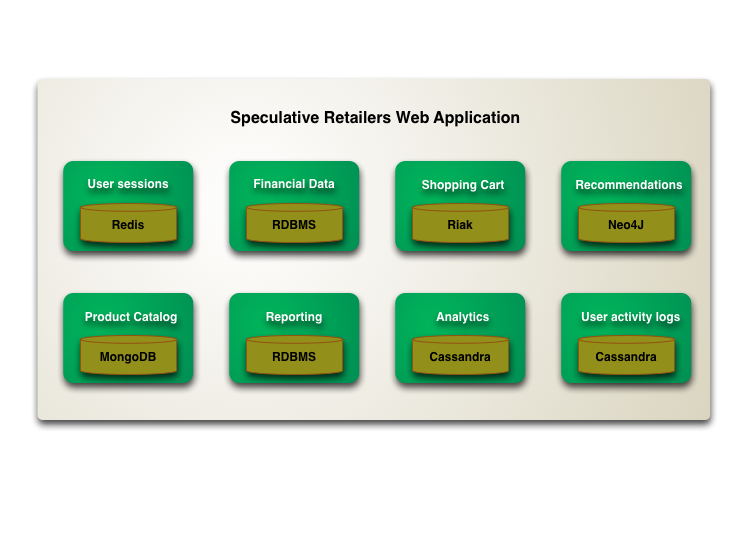
\includegraphics[width=1.0\linewidth]{polyglot.png}
\end{figure}
\end{frame}

%------------------------------------------------
\begin{frame}
\frametitle{Caracteristicas}
\begin{columns}[c]

\column{.45\textwidth} % Left column and width
\begin{enumerate}
\pause
\item Document-Oriented Storage
\pause
\item Full Index Support
\pause
\item Replication
\pause
\item Auto Sharding
\pause
\item Querying
\pause
\item Map Reduce
\pause
\item GridFS
\pause
\item \textbf{Other more...}
\end{enumerate}
\column{.5\textwidth} % Right column and width
\begin{itemize}
\item MMS.
\item Partner with MongoDB.
\item Multiples drivers.
\end{itemize}
\end{columns}
\end{frame}

%------------------------------------------------
\begin{frame}
\frametitle{Insert Find Update Remove (CRUD)}
\pause
\begin{block}{\textbf{I}FUR}
db.meetups.insert(\{"name":"mongoosejs","place":"Ruta N"\})
\end{block}
\pause
\begin{block}{I\textbf{F}UR}
db.meetups.find(\{"name":"mongoosejs"\})
\end{block}
\pause
\begin{block}{IF\textbf{U}R}
db.meetups.update(\{"name":"mongoosejs"\},
\{\$set:\{"description":"Ruta N, piso 0."\}\})
\end{block}
\pause
\begin{block}{IFU\textbf{R}}
db.meetups.remove(\{"name":"mongoosejs"\})
\end{block}
\end{frame}

%------------------------------------------------
\section{Javascript}
%------------------------------------------------
\begin{frame}
\frametitle{NodeJS - IOJS}
NodeJS es una plataforma de javascript construida sobre el "motor" V8 de Chrome.
{\color{blue}\url{https://nodejs.org//}}
\pause
\\~\\
IOJS es un fork de NodeJS. Implementando ES6 y desarrollado bajo un modelo de gobierno abierto.
{\color{blue}\url{https://iojs.org//}}
\end{frame}
%------------------------------------------------	
\section{Mongoose}
\begin{frame}[fragile]
\frametitle{Mongoose}
Un driver de MongoDB con NodeJS
\pause
\\~\\
\newcommand{\shellcmd}[1]{\\\indent\indent\texttt{\footnotesize\# #1}\\}
  \noindent instalaci\'on (En el directorio del proyecto.)
  \shellcmd{npm install mongoose --save}
\end{frame}

\begin{frame}
\frametitle{Entendiendo mongoosejs}
\begin{columns}[c]
\column{.3\textwidth} % Left column and width
Esquema
\column{.6\textwidth} % Right column and width
Un esquema es mapeado como una colecci\'on en MongoDB y 
define la forma de los documentos  con esa colecci\'on.
\end{columns}
\end{frame}

\begin{frame}[fragile]
\frametitle{Schema}
\medskip
\begin{lstlisting}
var mongoose = require('mongoose');
var schema = mongoose.schema;
var userSchema = Schema({
  firstName:String,
  lastName:String,
  telefones:{
    primary:String,
    secundary:String
  },
  hobbies:Array
});

\end{lstlisting}
Tipos: Number, Date, Buffer, Boolean, mixed and ObjectId.
\end{frame}

\begin{frame}
\frametitle{Entendiendo mongoosejs}
\begin{columns}[c]
\column{.3\textwidth} % Left column and width
modelos
\column{.6\textwidth} % Right column and width
Un modelo es un constructor compilado de nuestra definici\'on de esquema.
y representan los documentos que pueden ser guardados y recuperados de la base de datos.
\end{columns}
\end{frame}

\begin{frame}[fragile]
\frametitle{Model}
\medskip
\begin{lstlisting}
var User = mongoose.model('User',userSchema);
\end{lstlisting}
Ya tenemos a User listo para Insertar, encontrar, actualizar y eliminar.
Pero adem\'as, le podemos crear nuestras propias acciones al schema.

\begin{lstlisting}
userSchema.methods.findSimilarLastNames = function (cb) {
  return this.model('User').find({ lastName: this.lastName }, cb);
}
\end{lstlisting}
\end{frame}

\begin{frame}[fragile]
\frametitle{Metodos estaticos}
Statics
\\~\\
Agregar metodos estaticos a un modelo es simple.
\medskip
\begin{lstlisting}
userSchema.statics.findByName = function (name, cb) {
  this.find({ firstName: new RegExp(name, 'i') }, cb);
}
\end{lstlisting}
\end{frame}

\begin{frame}[fragile]
\frametitle{Indexes}
Los indices se pueden definir a nivel de esquema o a nivel de campo.
\\~\\
Campo
\begin{lstlisting}
firstName:{type:String, index:true}
\end{lstlisting}
Esquema
\begin{lstlisting}
animalSchema.index({firstName:1});
\end{lstlisting}
\end{frame}

\begin{frame}
\frametitle{Virtuals}
\begin{columns}[c]
\column{.3\textwidth} % Left column and width
get - set
\column{.6\textwidth} % Right column and width
Los metodos virtuales no se pueden persistir.
\end{columns}
\end{frame}

\begin{frame}
\frametitle{Comunidad}
\begin{enumerate}
\item Meetup: medellinjs  - mongodbmedellin
\pause
\item Twitter: @medellinjs - @mongodbmedelln
\pause
\item Facebook: /mongodbmedellin
\pause
\item gitter (chat): https://gitter.im/coljs/medellinjs
\pause
\item gitter (chat): https://gitter.im/MongoDBMedellin/Meetup
\end{enumerate}
\end{frame}
%------------------------------------------------	
\begin{frame}
\frametitle{Donde aprender}
\footnotesize{
\begin{thebibliography}{99} % Beamer does not support BibTeX so references must be inserted manually as below
\bibitem[]{p1} javascript (nodeJS)
\newblock http://nodeschool.io//
\end{thebibliography}
}

\footnotesize{
\begin{thebibliography}{99} % Beamer does not support BibTeX so references must be inserted manually as below
\bibitem[]{p1} MongoDB
\newblock https://university.mongodb.com/
\end{thebibliography}
}
\end{frame}

%------------------------------------------------
\begin{frame}
\frametitle{Preguntas}
\end{frame}

%------------------------------------------------
\begin{frame}
\Huge{\centerline{Gracias !!! =)}}
\end{frame}
%----------------------------------------------------------------------------------------

\end{document} 
